%%% Fiktivní kapitola s ukázkami citací

\chapter{Analýza}

\section{The Resource Description Framework}

Na internete nájdeme obrovské množstvo informácii o zdrojoch. Zdrojom môže byť čokoľvek. Napríklad dokument, človek alebo hmatateľný objekt.
Informácie o zdrojoch je potrebné spracovávať rôznymi aplikáciami, nie len umožniť človeku tieto informácie čítať. Na to bol úmyselne navrhnutý
The Resource Description Framework.

The Resource Description Framework (v skratke označovaný ako RDF) je framework, ktorého zámer je vyjadriť informácie o zdrojoch. RDF poskytuje bežné obecne známy
prístup ako vyjadrovať informácie. Vďaka tomu si dokážu rôzne aplikácie navzájom vymieňať
informácie a to bez straty významu informácii.

RDF môže byť použitý na prepájanie dát na internete. Uveďme si jednoduchý príklad.
Majme dáta reprezentujúce mesto Praha, v ktorých je zahrnutá informácia, že Praha je hlavným mestom
Českej republiky. Tato informácia môže byť vyjadrená ako odkaz na dáta reprezentujúce
Českú republiku. Získanie týchto dát nám poskytne viac informácii o Českej republike. Takto prechádzaním na odkazy vedúce k ďalším zdrojom si dokáže človek alebo automaticky proces
aplikácie zbierať informácie o rôznych veciach. Takéto využitie sa často kvalifikuje ako
Linked Data [LINKED-DATA].

\subsection{RDF Dátový Model }

Pre vyjadrovanie informácii v RDF je potrebné požívať obecný formát,
ktorý vedia stroje čítať. V RDF je formát štruktúrovaný ako nasledujúca trojica:

\begin{code}
    <predmet> <predikát> <objekt>
\end{code}

Formát vyjadruje vzťah medzi predmetom a objektom. Obe sú zdroje, ktoré
nejako spolu súvisia. Predikát v tomto formáte vyjadruje vzťah medzi predmetom a objektom.
Tento vzťah je formulovaný smerom od predmetu ku objektu a v RDF sa nazýva ako vlastnosť.
Pretože na vyjadrenia v RDF sa používa štruktúra o troch prvkov tak nazývame tieto vyjadrenia "trojica" (anglicky “triple”)


Pre lepšiu predstavu uveďme zopár konkrétnych príkladov trojíc:
\begin{code}
    <Karlov most> <je pomenovaný po> <Karol IV>
    <Karlov most> <je> <kamenný most>
    <kamenný most> <je> <most>
    <kamenný most> <je z materiálu> <kameň>
\end{code}

Konkrétny zdroj je často odkazovaný vo viacerých trojiciach. Taktiež v jednej trojici môže vystupovať ako predmet a v inej ako objekt. To nám umožni
získavať prepájanie medzi trojicami čo dáva RDF dôležitú a silnú schopnosť zbierať informácie.

Trojice vieme vizuálne vyjadriť ako spojený graf. Tento graf je tvorený vrcholmi, ktoré
reprezentujú predmety a objekty. Hrany medzi vrcholmi reprezentuje predikát.

Keď sú informácie vyjadrené v spojenom grafe, tak môžeme na nich použiť SPARQL pre získavanie informácii.

\subsection{Typy RDF dát }
V trojici sa vyskytujú tri typy dát: IRI, literál a prázdny vrchol

\textbf{IRI}

Úlohou IRI ("International Resource Identifier") je
identifikovať zdroj. Poznáme aj URL (Uniform Resource Locators) na adresovanie
webových stránok. URL je jedna z foriem IRI. Ostatné formy IRI identifikujú zdroj bez
uvedenia kde je zdroj umiestnený alebo ako k nemu pristupovať.
IRI je zovšeobecnením identifikátora URI (Uniform Resource Identifier),
ktorý umožňuje použitie znakov iných ako ASCII v reťazci znakov IRI.

URI sa môže vyskytovať na všetkých troch pozíciách v trojici.

\textbf{Literal}

Jednoducho povedané literal je hodnota, ktorá nie je URI. Literalom môžu byť textové reťazce, dátumy" alebo čísla.
S literalom sa viaže aj jeho dáta typ. Ten pomáha pri správnom interpretovaní hodnoty.

Literal sa môže vyskytnúť v trojici iba ako objekt. To nám reprezentuje také hodnoty objektov, ktoré
nie sú nijaký iný zdroj, ale iba napríklad číslo, text alebo dátum.

\textbf{Prázdny vrchol}
Niekedy je užitočné rozprávať o zdrojoch bez toho aby sme sa zaoberali
použitím  globálneho identifikátora. Ako príklad si uvedieme obraz “Mona Lízi”.
Tento obraz má svoj identifikátor, ale na obraze v pozadí môžeme vidieť strom, ktorý nemá svoj identifikátor,
ale vieme o aký je to strom. Zdroje bez globálneho identifikátora ako tento strom môžeme v RDF
reprezentovať ako prázdny vrchol.
Tento prázdny vrchol je ako jednoduchá premenná v algebre. Tá nám predstavuje nejakú vec bez toho aby sme uviedli aká je hodnota tejto veci.

Prázdny vrchol sa môže vyskytovať na pozícii predmetu a objektu.

\subsection{Viaceré grafy}
V praxi keď tvoríme a spravujeme informácie, tak by sa nám zišiel mechanizmus, vďaka ktorému by
sme vedeli hovoriť o nejakej podmnožine kolekcie trojíc. Z toho dôvodov RDF poskytuje mechanizmus
na zoskupenie vyjadrený RDF do viacerých grafov a priradiť takému grafu IRI. Viaceré grafy sú nedávnym
rozšírením RDF dátového modelu.

Viaceré grafy v RDF tvoria RDF dataset, čo je kolekcia RDF grafov.
Viaceré grafy boli prvý krát predstavené v RDF dotazovacom jazyku SPARQL.

\subsection{RDF slovníky}
RDF dátový model poskytuje spôsob ako o zdroju uviesť vyjadrenie.
Problémom je, že tento model netvrdí nič o tom čo konkrétnu IRI znamenajú. Z tohto dôvodu
sa v praxi zvykne RDF kombinovať so slovníkmi alebo inými konvenciami, ktoré poskytnú
sémantickú informáciu o zdrojoch.

Pre podporu definovať slovník poskytuje RDF jazyk RDF Schéma.
Tento jazyk nám dovoľuje definovať sémanticky význam RDF dát.
RDF Schéma je sémantické rozšírenie RDF.

V RDF Schéme nájdeme systém tried a vlastnosti, ktorý je podobný systému aký sa používa v objektovo
orientovaných programovacích jazykov. Na rozdiel od iných takýchto
systémov, kde sa trieda definuje z hľadiska vlastnosti, sa
v RDF Schéme systém odlišuje pravé v tom, že používa pojem triedy na špecifikáciu kategórii, ktoré môžeme
použiť na klasifikáciu zdrojov. Vzťah medzi triedou a jej inštanciami je daný prostredníctvom vlastnosti type.
Pomocou RDF Schémy vieme vytvárať hierarchiu tried, pod-tried a vlastnosti, pod-vlastnosti.
Taktiež je možné definovať typové obmedzenia pre predmety a objekty jednotlivých trojíc prostredníctvom
obmedzení domény a zadaniu rozsahu.

Pomocou RDF Schémy vieme zostaviť model údajov RDF.

Pre lepšiu predstavu uveďme jednoduchý neformálny príklad:
\begin{code}
    <Pražský hrad> <typ> <Hrad>
    <Hrad> <pod-trieda> <opevnenie>
    <nachádza v správnom územnom celku> <typ> <vlastnosť>
    <nachádza v správnom územnom celku> <doména> <správny územný celok>
    <nachádza v správnom územnom celku> <rozsah> <správny územný celok>
    <nachádza v správnom územnom celku> <pod-vlastnosť> <lokácia>
\end{code}


\section{Wikidata}
Wikidata sú bezplatná, vedomostná a sekundárna databáza obsahujúca otvorené dáta.
Tuto databázu môžu čítať a upravovať ľudia a aj stroje.
Pojmom “sekundárna databáza” myslíme, že Wikidata neobsahujú iba čisto natvrdo vyjadrené informácie,
ale aj ich zdroje a prepojenia na iné databázy. Z toho plynie rozmanitosť a dostupnosť poznatkov.

Wikidata fungujú ako centrálne úložisko pre štruktúrované údaje pre partnerské projekty
ako napríklad Wikipédia.

Wikidata sú taktiež mnoho-jazyčné, teda informácie tu nájdeme v rôznych jazykov.

Wikidata pozostávajú hlavne z položiek, ktoré sa označujú ako “items”.
Každá položka má štítok (label), popis (description) a číslo udávajúce počet aliasov.

Štítok je najbežnejšie meno označujúce danú položku, ktorá je dobre známa pod
týmto označením. Štítok zároveň nemusí byť jedinečný. Viacero položiek môže mať rovnaké pomenovanie.

Popis na Wikidatach je krátky opis, fráza ktorou úlohou je odlíšiť položky s rovnakými alebo
podobnými štítkami. Popis nemusí byť jedinečný rovnako ako štítok, ale žiadne dve položky nemôžu mať zároveň rovnaký štítok a aj popis.

Alias je alternatívne meno, alebo označenie položky, pod ktorým je položka taktiež známa.
Na Wikidatach môžeme vyhľadávať položky podľa štítku alebo aliasu.

Aby vedeli Wikidata jednoznačne od seba položky jednoznačne odlíšiť, tak každá položka má svoj unikátny identifikátor.
Tento identifikátor obsahuje na začiatku vždy veľké písmeno Q a za ním nasleduje číslo. Tento identifikátor označme ako "QNumber".
Napríklad mesto Praha ma identifikátor Q1085.

Vyjadrenie (anglicky statement) je trojica predmet, predikát a objekt reprezentujúci trojicu z RDF. Statement vyjadruje informácie, zaznamenané na Wikidatach, o položke.
Statment pozostáva z dvojice vlastnosť (anglicky property) a hodnota (anglicky value).

Každá vlastnosť reprezentuje informáciu a ma k sebe priradenú aspoň jednu hodnotu, ale môže nadobúdať aj viacero.
Vlastnosti na Wikidatach majú taktiež
ako položky svoj identifikátor, ktorý je rovnaký ako u položiek až nahradenie písmena Q za písmeno P. Napríklad vlastnosť "lokácia" ma identifikátor P276.

Hodnoty v statment-och sú dáta opisujúce položku. Ako už bolo spomenuté vlastnosť
ak je to rozumné môže nadobúdať viacero hodnôt. Napríklad osoba môže mat vlastnosť "deti", kde hodnota
je odkaz na položku reprezentujúcu dieťa danej osoby. Osoba ale môže mať viacero deti, a teda je
povolene aby vlastnosť mohla mať viacero hodnôt.
Ideálne je, keď každá vlastnosť ma iba jedno hodnotu. Napríklad vlastnosť "populácia" by mala mať len jednu hodnotu,
ktoré udáva počet obyvateľov. Problém ale je, že to tak vždy nie je. Aj takáto vlastnosť môže nadobúdať viaceré hodnoty,
z dôvodu, že rôzne zdroje uvádzajú rôzne hodnoty. Preto sa k týmto hodnotám
priradzujú ďalšie pridané informácie poskytujúce. Sú to kvalifikácie (anglicky qualifiers), ranky (Ranks) a referencie (references).

Referencie odkazujú na konkrétny zdroj, ktorý poskytol Wikidatam hodnotu pre daný statmnent.

Ranky poskytujú mechanizmus anotovať viaceré hodnoty statmentu. Na Wikidatach sa používajú tri druhy rank-ov:

\begin{enumerate}
    \item preferovaný rank -  hodnota najlepšie opisujúca danú vlastnosť
    \item normalny rank - defaultne nastavený rank
    \item zastaraný (deprecated) rank - hodnota s týmto rankom je zastaraná a najskôr neopisuje dobre vlastnosť
\end{enumerate}

Kvalifikácie taktiež ako ranky a referencie umožňujú expandovať, anotovať statement. Statement je iba
dvojica vlastnosť a hodnota a pre spresnenie hodnoty, respektíve pre ďalší opis vlastnosti sa používajú kvalifikácie.

Každá vlastnosť nadobúda hodnoty určitého dátového typy. Uveďme niektoré z nich, ktoré sú pre naše využitie najdôležitejšie:

\begin{enumerate}
    \item Kvantitatívne hodnoty - sú uvedené ako desatinné číslo.
          Vlastnosti tohto dátového typu by mali obsahovať aj informácie o obmedzeniach ako
          maximálna a minimálna možná číselná hodnota, ktorú môže číselná hodnota nadobúdať. Keď vlastnosť udáva hodnotu, ktoré môže byť
          uvedené v nejakej meracej jednotke (anglicky unit),
          tak vlastnosť by mala obsahovať obmedzenie, ktoré udáva v akých jednotkách sa môže hodnota vyjadriť.
    \item Item  hodnoty -  najbežnejší typ hodnoty na Wikidatach, kde hodnota je referencia
          na inú položku na Wikidatach. Vlastnosti tohto dátového typu by mali obsahovať obmedzenia, ktoré udávajú  aké položky sú prijateľné, neprijateľné ako hodnoty v pre danú vlastnosť.
    \item Textová hodnota - textový reťazec vyjadrený ako string.
    \item Časová hodnota - bod v čase. Týmto bodom môže byť napríklad dátum, rok, storočie alebo milénium.
    \item Geografické súradnice - dvojica čísel, ktoré vyjadrujú súradnice poloźky.
\end{enumerate}

\begin{figure}[p]\centering
    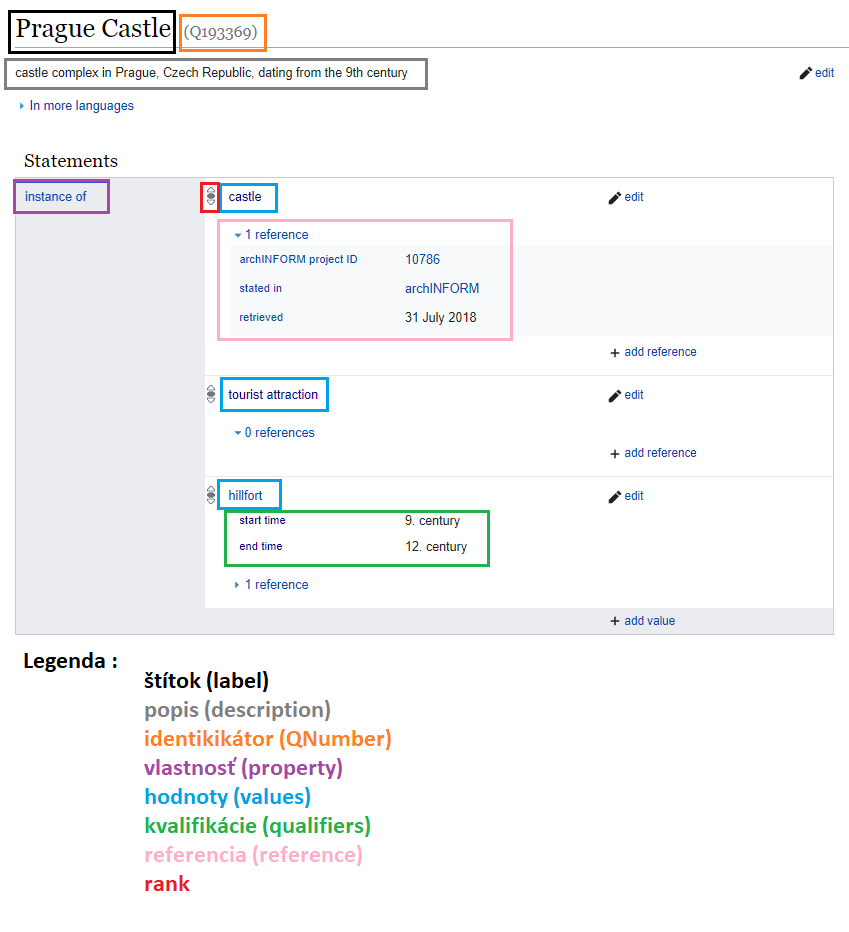
\includegraphics[width=140mm, height=160mm]{../img/ukazka-wikidata.png}
    \caption{Ukažka Wikidát s popisom}
\end{figure}

\section{Wikidata Query Service }
Wikidata obsahujú obrovské množstvo dát. Pre získanie konkrétnych dát je potrebne Wikidatam položiť otázku.
Jazyk v ktorom sa formulujú otázky na databázy, respektíve povedané dotazy,  je SPARQL.
Dotazom rozumieme špeciálnu formu otázky, ktorej
stroj rozumie a dokáže na ňu poskytnúť odpoveď.

Wikidata Query Service (WDQS) je softwarový balíček a zároveň verejne dostupná služba navrhnutá
na poskytovanie koncového bodu SPARQL, ktorý umožňuje sa pýtať na dáta poskytujúce Wikidatami.
WDSQ pracuje na dátach reprezentovaných v RDF formáte.

V nasledujúcich pod-sekciách si ukážeme základy potrebne na formovanie dotazov  v jazyku SPARQL.

\subsection{SPARQL pre Wikidata}
Základom je trojica predmet, predikát a objekt, ktoré reprezentujú statement na Wikidatach.
Statement "Zem sa nachádza v Mliečnej dráhe" pozostáva z predmetu "Zem" (Q2), predikátu "
nachádza sa v" (P276) a objektu "Mliečna dráha (Q321). Tento statement sa dá vyjadriť ako tri URI.

\begin{code}
    <http://www.wikidata.org/entity/Q2> // predmet
    <http://www.wikidata.org/prop/direct/P276> // predikát
    <http://www.wikidata.org/entity/Q321>. // objekt
\end{code}

Zakaždým písať všetko ako URI je príliš zdĺhavé,
a preto sa zaviedli prefixy.
Predmet a predikát musia byť vždy uložené ako URI. Objekt je buď URI alebo literal. Zoberme si "Zem" (Q2) , ktorá je uložená ako
<http://www.wikidata.org/entity/Q2>. Vďaka prefixom vieme dlhé URI nahradiť za krátku formu: wd:Q2.

Statement s použitím prefixov môžeme vyjadriť nasledovne:

\begin{code}
    wd:Q2  wdt:P276  wd:Q321 .
\end{code}

Entita (wd:) reprezentuje entitu na Wikidatach, respektíve položku, čo má priradený QNumber.
Prefix wdt: ukazuje priamo na objekt. WDSQ rozumie aj ďalším iným prefixom ako napríklad p, ps a pq.

Jednoduchý SPARQL dotaz pre Wikidata, ktorý vráti všetky entity, ktoré sú inštanciou triedy “hrad” môže vyzerať následovne:

\begin{code}
    SELECT ?item
    WHERE
        {
            ?item wdt:P31 wd:Q23413. # položka musí byť hrad
        }
\end{code}

Za SELECT nasledujú výpis premenných, ktoré má dotaz vrátiť ako výsledky.
Premenná vždy začína s prefixom ?.
WHERE blok obsahuje obmedzenia na dotaz vyjadrené ako trojice.
Keď sa spustí dotaz, WDSQ služba do premenných dosadí skutočne hodnoty, podľa trojíc uvedených
v dotaze. Vo vyššie uvedenom príklade sa do premennej ?item dosadia všetky položky, ktoré sú inštanciou triedy hradu.

Dáta na Wikidatach sú usporiadané v hierarchii. Položka je inštanciou nejakej inej položky reprezentujúcu triedu.
Trieda je pod-trieda inej triedy. Vlastnosť "je inštanciou" označujeme P31 a "je pod-triedou" označujeme P279.

\subsection*{Cesta}
Často do premennej dosadzujeme inštancie triedy, ktorá je ale pod-triedou určitej triedy.
V takom prípade aby sme nemuseli písať viacero trojíc môžeme predikát vyjadriť ako “cestu” medzi dvoma položkami. Pridať element cesty sa dá pomocou "/".
Predikátom vyzerá nasledovne: wdt:P31/wdt:P279

Tato cesta vyjadruje len, že položka je inštanciou triedy, ktorá je pod-triedou inej položky.
Cesta sa da predlžiť.
Aby sme ale zbytočne neopakovali elementy v ceste a nemuseli presne špecifikovať dĺžku cesty, tak za element cesty sa dá použiť
symbol “*” alebo symbol “+”.

Symbol * vyjadruje "nula alebo viac ako tento element" a + vyjadruje "jeden alebo viac ako tento element".

\subsection*{LIMIT a ORDER BY}
Za blokom WHERE{} môžeme pridať:
\begin{itemize}
    \item LIMIT - vyjadruje maximálny počet vrátených výsledkov. Napríklad LIMIT 10 vráti iba
          10 výsledkov, aj keď ich môže byť viacej.
    \item ORDER BY - zoradí výsledky dotazu podľa výrazu alebo premennej, ktorú vieme zabaliť do ASC() alebo DESC(), čo určí poradie zotriedenia.
\end{itemize}

\subsection*{OPTIONAL a MINUS}

Vrátene výsledky musia spĺňať všetky trojice.
Je užitočne niekedy ale označiť trojicu za voliteľnú. V takom prípade sa vrátia aj výsledky nespĺňajúce
danú trojicu. Voliteľné trojice sa píšu do vnútra bloku OPTIONAL {}.

Na druhú stranu blok MINUS {} umožňuje vybrať tie výsledky, ktoré nezodpovedajú trojiciam vo vnútri bloku.
Používa sa keď je jednoduchšie zadať, že výsledky nemajú spĺňať trojice vo vnútri bloku ako vytvárať negáciu.

\subsection*{VALUES}
V SPARQL dotazov vieme do premennej manuálne priradiť položky. Formát je nasledovný:
\begin{code}
    VALUES ?item { wd:Q2 wd:Q513 }
\end{code}
Teraz premenná ?item obsahuje dve položky.

\subsection*{FILTER}
Pre filtrovanie položiek na základe výrazu sa používa blok FILTER(), kde do vnútra vložíme výraz.
Tento výraz musí vrátiť pravdivostnú hodnotu True alebo False.

Vo výraze sa používajú bežne matematické operátory ako +, -, *, /. Výrazy na porovnávanie
<, > , = , >= , <=. Výrazy sa dajú kombinovať použitím logických operátorov.

Taktiež je možne odfiltrovať konkrétne položky.
\begin{code}
    FILTER ( ?item not in ( wd:Q193369) ) # odfiltruj Pražský hrad.
\end{code}

\subsection*{GROUP BY}
Niekedy nechceme aby dotaz vrátil výsledky, ale napríklad počet výsledkov.
Na to slúžia agregované funkcie.

Prehlaď agregovaných funkcií:
\begin{enumerate}
    \item COUNT - počet elementov v premennej.
    \item SUM - suma všetkých hodnôt v premennej.
    \item AVG - priemer všetkých hodnôt v premennej.
    \item MIN, MAX - minimum, alebo maximum z hodnôt.
    \item SAMPLE - ľubovoľný jeden element z premennej.
    \item GROUP CONCAT - zreťazenie elementov.
\end{enumerate}

Aby sa v dotaze mohla použiť agregovaná funkcia na premennú, musí byť táto premenná braná ako skupina.
To dosiahneme tým, že za blok WHERE {} sa pridá GROUP BY a nasleduje výpis premenných branných ako skupina.

\subsection*{Kvantifikátory}

Prefix wdt: ukazuje priamo na objekt v statement-e. Prefix p: neukazuje priamo na objekt, ale
na statement uzol. Tento uzol je následne predmetom v ďalšej trojici. Pre tuto trojicu vieme
použiť prefix ps:, ten ukazuje na objekt a prefix pq:, ktorý ukazuje na kvalifikátor.

Príklad k získaniu populácie mesta Praha, zároveň so získaním dátumu namerania populácie vyjadrený ako kvalifikátor hodnoty: 
\begin{code}
    SELECT ?population ?date
    WHERE
        {
            # Praha , populácia , statement uzol
            wd:Q1085 p:P1082 ?populationNode.
            # statement uzol , populácia , premenná pre populáciu
            ?populationNode ps:P1082 ?population.
            # statement uzol , “k dátumu” , premenná pre vlasnosť
            ?populationNode pq:P585 ?date.
        }
\end{code}

\subsection{Label service}
Label service je užitočná služba pre získavanie štítkov položiek, pretože 
znižuje náročnosť dotazov, ktoré bez nej by inak boli náročnejšie pre dosiahnutie rovnakého efektu. 

WDQS služba podporuje túto službu, ktorá rozširuje štandardné schopností SPARQL. 

Služba vieme použiť v dvoch režimoch. Automaticky a manuálny. 

V automatickom režim stačí do dotazu pridať iba šablónu služby, kde je potrebne uviesť 
jazyk, ktorý služba bude preferovať. Následne WDQS automaticky vygeneruje štítky na základe: 
\begin{enumerate}
    \item Ak ma neviazaná premenná v SELECT bloku názov “?<názov premennej>Label”, potom do nej WDQS vytvorí štítok 
          (rdfs:label) pre položku v premennej “?<názov premennej>”. 
    \item Ak ma neviazaná premenná v SELECT bloku názov “?<názov premennej>AltLabel”, potom do nej WDQS vytvorí alias 
          (skos:altLabel) pre položku v premennej “?<názov premennej>”. 
    \item Ak ma neviazaná premenná v SELECT bloku názov “?<názov premennej>Description”, potom do nej WDQS vytvorí popis 
          (schema:description) pre položku v premennej “?<názov premennej>”. 
\end{enumerate}

Je možne uviesť viac jazykov, ktoré sa zvažujú v poradí ako sú uvedene.
Za [AUTO LANGUAGE] WDQS automaticky nahradí jazyk momentálneho užívateľského rozhrania. 

Príklad automatického módu: 
\begin{code}
    SERVICE wikibase:label {
    bd:serviceParam wikibase:language "en" .
    }
\end{code}

Automatický režim kontroluje iba projekciu dopytu. 
Napríklad pri použití SELECT ?aLabel (SAMPLE(?bLabels) AS ?bLabel) WDQS rozpozná 
iba prvý štítok a teda v premennej ?bLabel nebude štítok. 
V takýchto prípadoch je potrebné použiť manuálny režim. 

V manuálnom režime je potrebne explicitne naviazať premenné štítkov v rámci servisného volania. 
\begin{code}
    SELECT *
    WHERE {
    SERVICE wikibase:label {
    bd:serviceParam wikibase:language "en, de" .
    wd:Q2 rdfs:label ?q2Label .
    wd:Q2 skos:altLabel ?q2Alt .
    wd:Q2 schema:description ?q2Desc .
    }
    }
\end{code}

\subsection{Geopriestorové vyhľadávanie - Around service }
Službu umožňujúcu vyhľadávať položky so súradnicami, ktoré sa nachádzajú v určitom okruhu 
od zadaného stredného bodu. 

Prvý riadok around služby musí byť vo formáte: ?item (ľubovoľný názov premennej) wdt:P625 ?location. 
Nájdene výsledky sa priradia do premennej ?item a do ?location sa priradia súradnice týchto položiek. 
Predikát wdt:P625 je získanie hodnoty vlastnosti zemepisné súradnice. 

Ďalšie parametre sú následovne: 
\begin{itemize}
    \item wikibase:center - bod okolo ktorého sa vyhľadáva. Buď sa poskytuje premenná obsahujúca 
          súradnice, alebo literal so súradnicami vo formáte textového reťazca: "Point( 
          <zemepisná šírky> 
          <zemepisná výška>)"^^geo:wktLiteral . 
    \item wikibase:radius - vzdialenosť od bodu v kilometroch, ktorá definuje kruh vyhľadávania. 
\end{itemize}

Nasleduje príklad dotazu, ktorý vyhľadá všetky hrady vzdialene 100 km od mesta Praha. 
\begin{code}
    SELECT ?place ?placeLabel ?location ?dist WHERE {
    # Praha súradnice
    wd:Q1085 wdt:P625 ?súradnicePrahy .
    SERVICE wikibase:around {
    ?item wdt:P625 ?location .
    bd:serviceParam wikibase:center ?súradnicePrahy .
    bd:serviceParam wikibase:radius "100" .
    }
    # Položka je hrad
    FILTER EXISTS { ?item wdt:P31/wdt:P279* wd:Q23413 }
    SERVICE wikibase:label {
    bd:serviceParam wikibase:language "en" .
    }
    }
\end{code}

\subsection{MediaWiki API Query Service}
MediaWiki API Query Service (MWAPI) dovoľuje zo SPARQL volať MediaWiki API a vrátiť výsledky naspať 
do SPARQL. 
Do dotazu sa služba zavolá použitím bloku SERVICE wikibase:mwapi {}. 
Do vnútra bloku sa vkladajú parametre služby. 
Parametre “wikibase:api” a “wikibase:endpoint” sú povinné parametre. “Endpoint definuju” koncového hostiteľa. 
“Api” definuje ktorá API bude na koncovom hostiteľovi vykonaná. 

Z default nastavený táto služba vracia všetky výsledky. Parametrom “wikibase:limit” sa dá nastaviť 
počet vrátených výsledkov. Má to rovnaký efekt ako LIMIT, ale ten sa aplikuje, až kde API volanie skonči a preto je vhodnejšie použiť tento parameter. 

Ostatné parametre začínajú prefixom 
“mwapi” ako napríklad mwapi:language "en", ktorý definuje jazyk dotazu. 

Pre definovanie výstupných parametrov, ktoré sa vrátia z volania API, to  
vyzerá nasledovne: 
\begin{code}
    ?item wikibase:apiOutput mwapi:title .
\end{code}

Do premennej “?item” sa dosadí výsledok definovaný výstupnou premennou "title". Je dôležite 
zdôrazniť, že použite výstupne parametre očakávajú prítomnosť určitých vstupných parametrov. 

Predikát “wikibase:apiOrdinal”, ktorý berie ako objekt pravdivostnú hodnotu, dovoľuje definovať 
výsledkom čísla poradia, ktoré sa nastavia podlá poradia aké originál API vráti. 

Ukážme si jednu konkrétnu podporovanú službu, ktorou je “EntitySearch”. 
Táto služba vyhľadáva Wikibase položky na základe názvu. 

Vstupne parametre pre túto službu sú: 
\begin{itemize}
    \item search - zadanie názvu, podľa ktorého sa vyhľadáva 
    \item language – jazyk použitý vo vyhľadávaný 
    \item limit - maximálny počet vrátených výsledkov 
    \item type 
\end{itemize}

Výstupne parametre pre túto službu sú: 
\begin{itemize}
    \item item - vracia položky ako objekt, ktorý môže byť predmetom v iných trojiciach 
    \item label - vráti iba štítok nájdených položiek 
\end{itemize}

Dotaz pre vyhľadanie všetkých hradov, ktoré v názve majú hrad by vyzeral nasledovne: 
\begin{code}
    SELECT * WHERE { 
    SERVICE wikibase:mwapi { 
    # koncový hostiteľ 
    bd:serviceParam wikibase:endpoint "www.wikidata.org"; 
    wikibase:api "EntitySearch"; # názov API služby 
    mwapi:search "castle"; # hľadané slovo 
    mwapi:language "en". # jazyk anglicky 
    # do ?item prirať nájdené položky 
    ?item wikibase:apiOutputItem mwapi:item. 
    # priradenie do ?num číslo poradia nájdenia v API 
    ?num wikibase:apiOrdinal true. 
    } 
    ?item wdt:P31/wdt:P279* wd:Q23413 # výsledok je hrad 
    } ORDER BY ASC(?num) 
\end{code}

\section{Wikimedia service}
Wikimedia prevádzkuje verejnú inštanciu WDQS. Služba je dostupná na URL http://query.wikidata.org/. 
Existuje GUI verzia a verejný SPARQL koncový uzol. 

GUI dovoľuje editovať a odoslať SPARQL dotaz na vyhľadávací nástroj. Výsledky sú zobrazene ako 
HTML tabuľka. 

SPARQL dotazy môžu byť odoslané na koncový uzol buď GET alebo POST metódou. Výsledky sú vrátene ako 
XML alebo vieme nastaviť formát JSON. 

Výsledky dotazu sú serializované ako jeden JSON objekt najvyššej úrovni. Objekt sa skladá 
z hlavičky "head" a výsledkov "results". 

Nasledujúci príklad ukazuje výsledok SELECT dotazu. 
\begin{code}
    {
    "head": { "vars": [ "book" , "title" ]
    } ,
    "results": {
    "bindings": [
    {
    "book": {
    "type": "uri" ,
    "value": "http://example.org/book/book6"
    } ,
    "title": {
    "type": "literal" ,
    "value": "Harry Potter and the Half-Blood Prince"
    }
    } ,
    ]
    }
    }
\end{code}
V hlavičke sú premenne Select-u v objekte 
s kľúčom “vars” a hodnotou reprezentujúcou pole premenných. V členovi výsledky je 
objekt s kľúčom “bindings” a hodnotou ,ktorá je pole obsahujúce výsledky. Každý výsledok je objekt, ktorý pozostáva 
z dvojíc kľuč a hodnota, kde kľuč je názov premennej a hodnota je objekt reprezentujúci hodnotu premennej. 